\section{Référence de la classe Iterateur}
\label{class_iterateur}\index{Iterateur@{Iterateur}}
Graphe d'héritage de Iterateur::\begin{figure}[H]
\begin{center}
\leavevmode
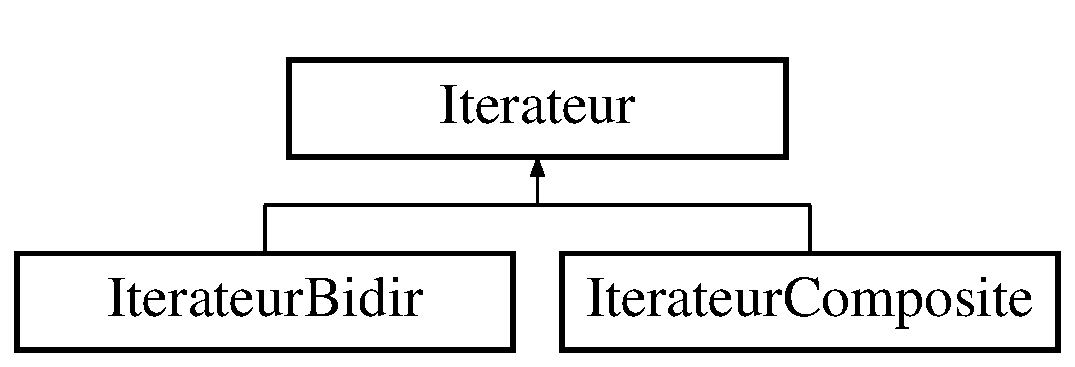
\includegraphics[height=2cm]{class_iterateur}
\end{center}
\end{figure}


\subsection{Description détaillée}
Interface qui définit les méthodes requises par un itérateur \char`\"{}unidirectionnel\char`\"{} simple. 

C'est également ici que se trouve la documentation sur le comportement attendu des implémentations. \subsection*{Fonctions membres publiques}
\begin{CompactItemize}
\item 
{\bf cle} ()
\begin{CompactList}\small\item\em Retourne la clé de l'élément courant de l'itérateur. \item\end{CompactList}\item 
{\bf courant} ()
\begin{CompactList}\small\item\em Retourne l'élément courant de l'itérateur. \item\end{CompactList}\item 
{\bf debut} ()\label{class_iterateur_1600a0b47466d85a5bb4af10a634b1ed}

\begin{CompactList}\small\item\em Place l'itérateur sur le premier élément. \item\end{CompactList}\item 
{\bf estDernier} ()
\begin{CompactList}\small\item\em Indique si l'élément courant de l'itérateur est le dernier. \item\end{CompactList}\item 
{\bf estPremier} ()
\begin{CompactList}\small\item\em Indique si l'élément courant de l'itérateur est le premier. \item\end{CompactList}\item 
{\bf estValide} ()
\begin{CompactList}\small\item\em Indique si la position courante de l'itérateur est valide, càd si un élément s'y trouve. \item\end{CompactList}\item 
{\bf fin} ()\label{class_iterateur_487fadeda3651d2add97628652fa6d1e}

\begin{CompactList}\small\item\em Place l'itérateur sur le dernier élément. \item\end{CompactList}\item 
{\bf Iterateur} (\$v\_\-oObjetAIterer)
\begin{CompactList}\small\item\em Constructeur. \item\end{CompactList}\item 
{\bf rechercher} (\$v\_\-Cle)
\begin{CompactList}\small\item\em Déplace l'itérateur jusqu'à un emplacement donné en fonction d'une clé. \item\end{CompactList}\item 
{\bf suiv} ()\label{class_iterateur_b49e1eadf71ee40a816ed2d5134e0ba7}

\begin{CompactList}\small\item\em Déplace l'itérateur d'une position vers l'avant. \item\end{CompactList}\item 
{\bf taille} ()
\begin{CompactList}\small\item\em Retourne le nombre d'éléments présents dans l'itérateur. \item\end{CompactList}\end{CompactItemize}


\subsection{Documentation des fonctions membres}
\index{Iterateur@{Iterateur}!cle@{cle}}
\index{cle@{cle}!Iterateur@{Iterateur}}
\subsubsection{\setlength{\rightskip}{0pt plus 5cm}Iterateur::cle ()}\label{class_iterateur_0bc2b87d3fa65a6df5c4d5134402d4ba}


Retourne la clé de l'élément courant de l'itérateur. 

\begin{Desc}
\item[Renvoie:]la clé de l'élément courant de l'itérateur \end{Desc}


Références OO::abstraite().\index{Iterateur@{Iterateur}!courant@{courant}}
\index{courant@{courant}!Iterateur@{Iterateur}}
\subsubsection{\setlength{\rightskip}{0pt plus 5cm}Iterateur::courant ()}\label{class_iterateur_525e78b4e7c5aec4cc4e8003ca9e730b}


Retourne l'élément courant de l'itérateur. 

\begin{Desc}
\item[Renvoie:]l'élément courant de l'itérateur \end{Desc}


Références OO::abstraite().\index{Iterateur@{Iterateur}!estDernier@{estDernier}}
\index{estDernier@{estDernier}!Iterateur@{Iterateur}}
\subsubsection{\setlength{\rightskip}{0pt plus 5cm}Iterateur::estDernier ()}\label{class_iterateur_b90977faf081ea8db8e56415e0bc9e2f}


Indique si l'élément courant de l'itérateur est le dernier. 

\begin{Desc}
\item[Renvoie:]{\tt true} si l'itérateur est positionné sur le dernier élément. Sinon {\tt false} \end{Desc}


Références OO::abstraite().\index{Iterateur@{Iterateur}!estPremier@{estPremier}}
\index{estPremier@{estPremier}!Iterateur@{Iterateur}}
\subsubsection{\setlength{\rightskip}{0pt plus 5cm}Iterateur::estPremier ()}\label{class_iterateur_6e49a71af6b96a13d20aa137ddd9ac2d}


Indique si l'élément courant de l'itérateur est le premier. 

\begin{Desc}
\item[Renvoie:]{\tt true} si l'itérateur est positionné sur le premier élément. Sinon {\tt false} \end{Desc}


Références OO::abstraite().\index{Iterateur@{Iterateur}!estValide@{estValide}}
\index{estValide@{estValide}!Iterateur@{Iterateur}}
\subsubsection{\setlength{\rightskip}{0pt plus 5cm}Iterateur::estValide ()}\label{class_iterateur_33d904743c851b2c959c514ecce923c8}


Indique si la position courante de l'itérateur est valide, càd si un élément s'y trouve. 

Cette fonction devrait toujours être appelée avant de récupérer une valeur ou une clé, afin de déterminer si le \char`\"{}pointeur\char`\"{} de l'itérateur est dans une position valide

\begin{Desc}
\item[Renvoie:]{\tt true} si la position courante de l'itérateur contient bien un élément valide. Sinon {\tt false} \end{Desc}


Références OO::abstraite().\index{Iterateur@{Iterateur}!Iterateur@{Iterateur}}
\index{Iterateur@{Iterateur}!Iterateur@{Iterateur}}
\subsubsection{\setlength{\rightskip}{0pt plus 5cm}Iterateur::Iterateur (\$ {\em v\_\-oObjetAIterer})}\label{class_iterateur_06ee079b3a67f46c02cd50ffab4913f7}


Constructeur. 

\begin{Desc}
\item[Paramètres:]
\begin{description}
\item[{\em v\_\-oObjetAIterer}]l'objet sur lequel aura lieu l'itération. Son type dépendra bien entendu de l'implémentation\end{description}
\end{Desc}
\begin{Desc}
\item[Note:]Selon l'implémentation, des paramètres supplémentaires pourront être acceptés ou requis \end{Desc}


Références OO::abstraite().\index{Iterateur@{Iterateur}!rechercher@{rechercher}}
\index{rechercher@{rechercher}!Iterateur@{Iterateur}}
\subsubsection{\setlength{\rightskip}{0pt plus 5cm}Iterateur::rechercher (\$ {\em v\_\-Cle})}\label{class_iterateur_b05ee08c7fc02253222a8f3604b65804}


Déplace l'itérateur jusqu'à un emplacement donné en fonction d'une clé. 

Si cette dernière n'existe pas, l'itérateur restera à la même position qu'avant l'appel

\begin{Desc}
\item[Paramètres:]
\begin{description}
\item[{\em v\_\-Cle}]la clé utilisée pour déplacer le \char`\"{}pointeur\char`\"{} interne de l'itérateur\end{description}
\end{Desc}
\begin{Desc}
\item[Renvoie:]{\tt true} si la clé recherchée existe bien dans la \char`\"{}collection\char`\"{} sur laquelle l'itérateur fonctionne, {\tt false} sinon \end{Desc}


Références OO::abstraite().\index{Iterateur@{Iterateur}!taille@{taille}}
\index{taille@{taille}!Iterateur@{Iterateur}}
\subsubsection{\setlength{\rightskip}{0pt plus 5cm}Iterateur::taille ()}\label{class_iterateur_40a496bef151a677b180e7805f106acd}


Retourne le nombre d'éléments présents dans l'itérateur. 

\begin{Desc}
\item[Renvoie:]le nombre d'éléments de l'itérateur \end{Desc}


Références OO::abstraite().

La documentation de cette classe a été générée à partir du fichier suivant :\begin{CompactItemize}
\item 
src/lib/std/{\bf Iterateur.php}\end{CompactItemize}
